% Created 2018-01-09 Tue 16:57
% Intended LaTeX compiler: pdflatex
\documentclass[11pt]{article}
\usepackage[utf8]{inputenc}
\usepackage[T1]{fontenc}
\usepackage{graphicx}
\usepackage{grffile}
\usepackage{longtable}
\usepackage{wrapfig}
\usepackage{rotating}
\usepackage[normalem]{ulem}
\usepackage{amsmath}
\usepackage{textcomp}
\usepackage{amssymb}
\usepackage{capt-of}
\usepackage{hyperref}
\pagenumbering{gobble}
\setlength{\parindent}{0em}
\usepackage{amsmath}
\usepackage{parskip}
\usepackage{titlesec}
\titlespacing{\section}{0pt}{\parskip}{-\parskip}
\titlespacing{\subsection}{0pt}{\parskip}{-\parskip}
\titlespacing{\subsubsection}{0pt}{\parskip}{-\parskip}
\usepackage{titlesec}
\usepackage[rmargin=1in, lmargin=1in, tmargin=1in, bmargin=0.7in]{geometry}
\date{}
\title{}
\hypersetup{
 pdfauthor={Teddy Groves},
 pdftitle={},
 pdfkeywords={},
 pdfsubject={},
 pdfcreator={Emacs 25.1.1 (Org mode 9.0.9)}, 
 pdflang={English}}
\begin{document}

\section*{Who is good at Test cricket?}
\label{sec:orgdb14a05}
Cricket fans often debate who is the best player, and these arguments
are pretty hard to settle as matches take so long, have so many
contributing factors, are pretty infrequent and involve a range of
skills. When rating football players at \href{http:www.footballradar.com}{Football Radar} we encounter
many of the same problems.

Below I use a similar approach to the one we currently use for
football to try and see which players are good at Test cricket.

\subsection*{Wait, what is `Test cricket'?}
\label{sec:orgc29a04f}
Cricket is a game with a well-deserved reputation for baffling
terminology, especially in its 5-day 'Test' format. For our purposes
the following description will more or less suffice:

\begin{itemize}
\item The game consists of lots of balls, arranged into up to 4 inningses
(2 per team).
\item Each ball (mostly) involves two players: batter vs. bowler.
\item The batter aims to score runs and not concede a wicket (in this case
they are out).
\item The bowler aims to take wickets and not concede runs.
\end{itemize}

\subsection*{Data}
\label{sec:org9a6a10b}
I downloaded data recording the outcomes of 809592 balls from 402 male Test
matches from the website \href{https://cricsheet.org/downloads/\#experimental}{cricsheet}, and condensed it into a table indicating how
many runs, balls and wickets happened for each bolwer/batter/innings
combination.

\subsection*{Model}
\label{sec:orgc35be06}
I used the following generalised linear models to describe the total number of
runs and wickets for a given combination \(c\) of bowler, batter and innings

\begin{gather}
\nonumber runs_{c} \sim NegativeBinomial(\lambda_{c}, \phi) \\ \nonumber
wickets_{c} \sim Binomial(balls_c, \eta_{c}) 
\end{gather}

where

\begin{align}
\nonumber\log(\lambda_{c}) &= \log(balls_{c}) \\ \nonumber &+
BaseRunRate_{innings_c} \\ \nonumber &+ RunAbilityBat_{batter_c} \\ \nonumber &-
RunAbilityBowl_{bowler_c} \end{align}
\begin{align}
\nonumber logit(\eta_{c}) &= BaseWicketRate_{innings_c} \\ \nonumber &+
WicketAbilityBat_{batter_c} \\ \nonumber &- WicketAbilityBowl_{bowler_c}
\end{align}

The binomial distribution for wickets in a combination implies a
logistic regression at the level of balls. The negative binomial
distribution allows the variance of the run distribution to differ
from the mean. I chose this method to take into account the
possibility of runs arriving irregularly in clumps rather than at a
constant rate.

Bowling and batting abilities have normal priors centered at zero, with
hierarchical standard deviations:

\begin{align}
\nonumber RunAbilityBat \sim Normal(0, \sigma_{RunBat}) \\ \nonumber
WicketAbilityBat \sim Normal(0, \sigma_{WicketBat}) \\ \nonumber RunAbilityBowl
\sim Normal(0, \sigma_{RunBowl}) \\ \nonumber WicketAbilityBowl \sim Normal(0,
\sigma_{WicketBowl}) \end{align}

Other parameters have weakly informative prior distributions.

This model specification implies that there is no systematic
correlation between the two dimensions of batting and bowling
ability. This choice is motivated by simplicity and the final results,
which suggest that the two dimensions are more or less uncorrelated
for both bowlers and batters.

\subsection*{Model checking}
\label{sec:orgd1018a5}
I generated simulated runs and wickets for each bowler/batter/innings
combination and compared these with the observed values, with the following
results:

\begin{center}
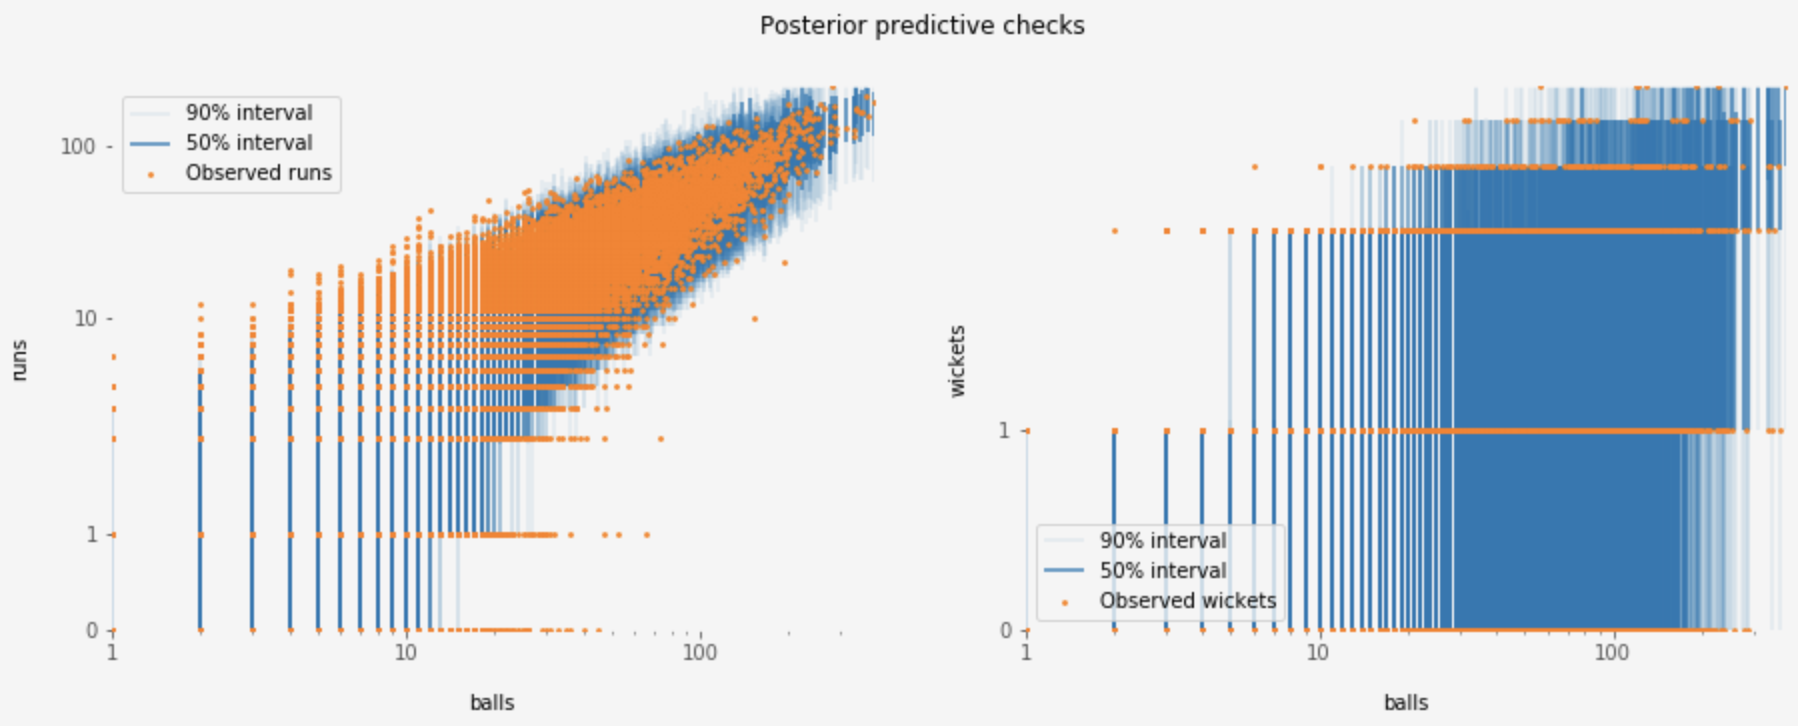
\includegraphics[width=.9\linewidth]{images/cricket_ppc.png}
\end{center}

Roughly the right amount of observed values lie outside the model's
90\% probable intervals. However, there is a pattern to the
discrepancies between observed and simulated runs - the points outside
the probable intervals occur almost exclusively for combinations with
lower numbers of balls. This makes intuitive sense, as the model does
not know that runs in cricket are mostly scored in increments of 1, 2,
4 and occasionally 6. The negative binomial likelihood is likely a
reasonable approximation to the truth when the number of balls is
high, but not when it is low.

This impression is backed up by the following histograms of observed
and simulated run and wicket counts:

\begin{center}
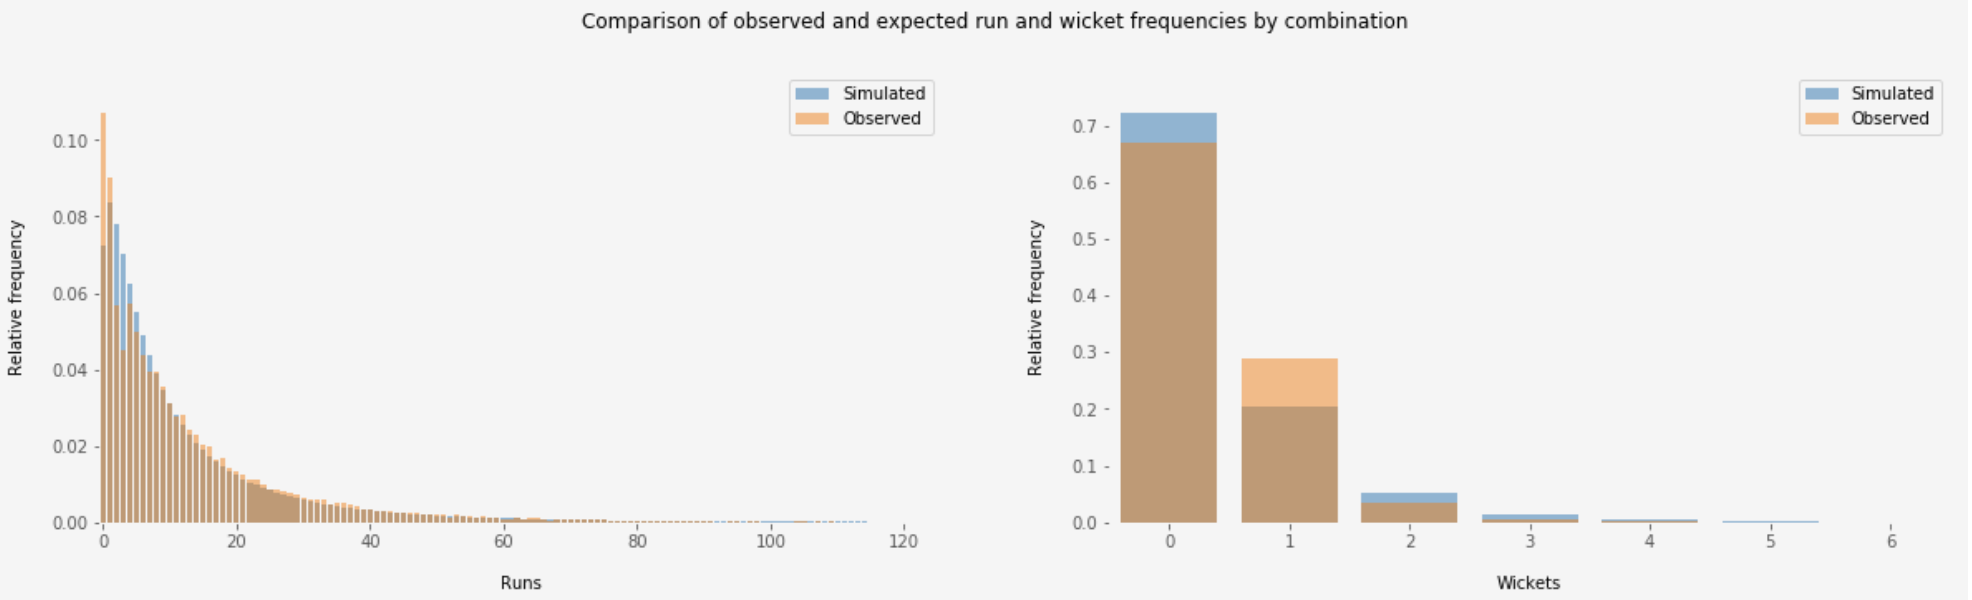
\includegraphics[width=.9\linewidth]{images/cricket_histograms.png}
\end{center}

Overall there seems to be room for improvement, but the model fits the
data well enough to make the results interesting.

\subsection*{Results}
\label{sec:org7f5f4df}
I made two charts - one plotting the posterior means of both abilities
for all players, with unusual players highlighted, and another with a
more detailed look at the players with the best wicket abilities.
\begin{center}
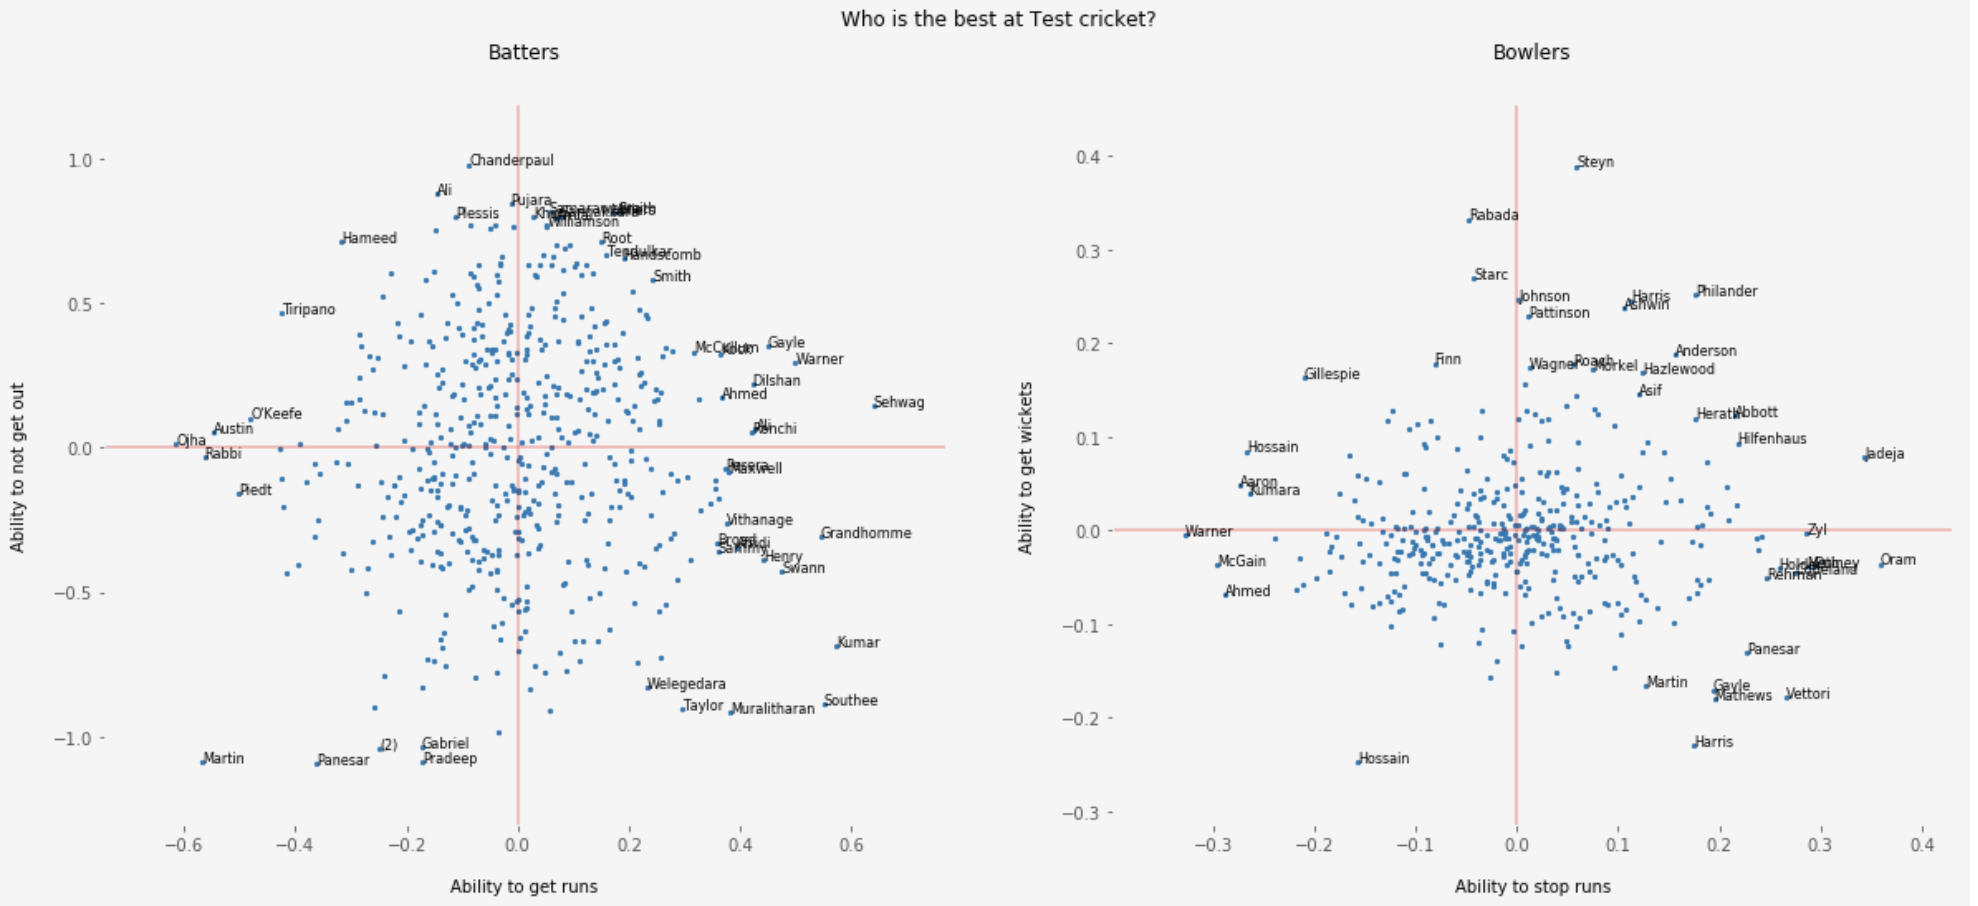
\includegraphics[width=.9\linewidth]{images/cricket_radar.png}
\end{center}

\begin{center}
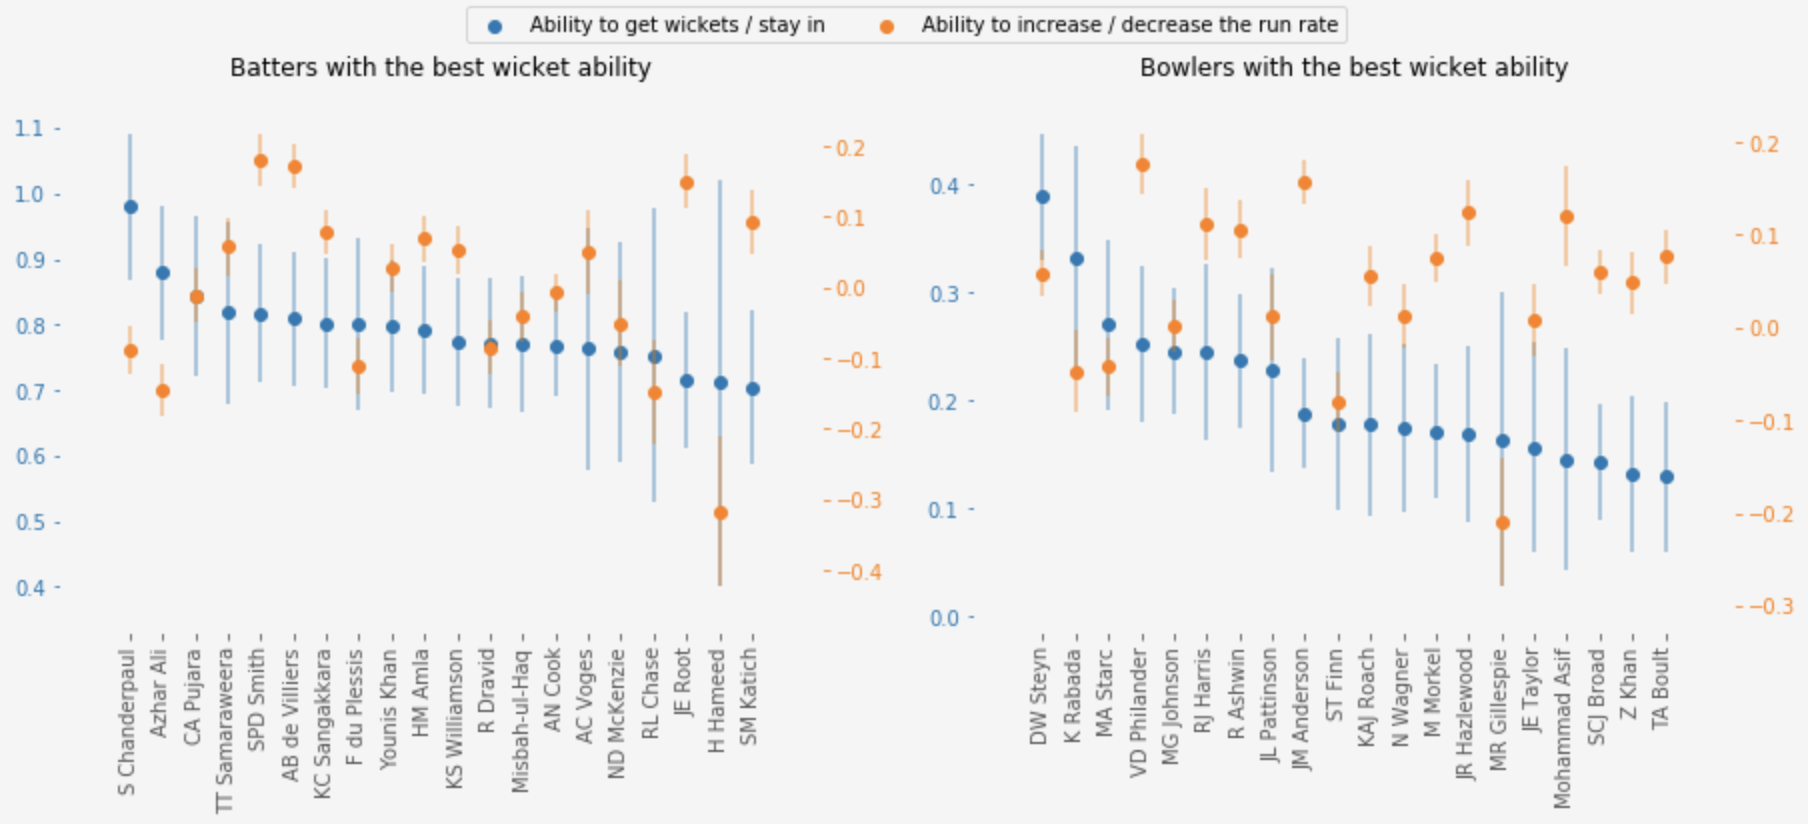
\includegraphics[width=.9\linewidth]{images/best_cricketers.png}
\end{center}

The model seems to have picked out good players fairly well. My
favourite players Mohammed Asif and Shivnarine Chanderpaul both make
it into the top twenty, and most of the other top-rated players seem
to be pretty good as well. I am slightly suspicious about the lack of
slow bowlers in the top 20 - apart from Ashwin they are all fast
bowlers who would probably do a lot of bowling when the ball is
relatively new - this suggests a natural way to extend the model.

\subsection*{Limitations}
\label{sec:org714200c}
I think this model works fairly well, but there are quite a few
limitations and extensions that would be interesting to investigate:

\begin{itemize}
\item The model misses lots of important factors, including fielding, ball age,
home advantage, change in ability over time, weather, stadium, game
state or stamina.
\item A ball can't usually involve both a wicket and a non-zero amount of
runs, but in the model it can.
\item There is probably a better way to describe the distribution of run
errors.
\item In order to say who is really the best player, run-rate ability
needs to be weighed against wicket ability.
\end{itemize}
\end{document}
